\documentclass[11pt]{article}

\usepackage[margin=1in]{geometry}
\usepackage[utf8]{inputenc}
\sloppy
\emergencystretch=3em
\usepackage{natbib}
\usepackage{graphicx}
\usepackage{hyperref}
\usepackage{booktabs}
\usepackage{pgfplots}
\pgfplotsset{compat=1.18}

\title{Knowing When to Look: Do LLMs Search When They Should for Security Facts?}
\author{Amit Porat (ID. 315390252)}
\date{Submitted as final project report for the NLP course, IDC, 2026}

\begin{document}

\maketitle

\section{Introduction}

People increasingly ask LLMs about security specifics: what a given CVE affects, whether a software package is safe, which setting hardens a system. A confident but wrong answer here is dangerous, and stronger models have not removed the risk \citep{abdullah2025security}. Modern models can also \textit{look things up} with a search tool — but they decide for themselves whether to use it. This raises a question almost no one has studied for security facts: \textbf{does the model choose to search at the right moments, and when it does search, does that actually stop it from giving a wrong answer?}

We study this through three questions. \textbf{RQ1}: does the model choose to search only when it doesn't already know the answer? \textbf{RQ2}: does giving the model a search tool change how it handles a fabricated CVE ID — rejecting the premise, fabricating a vulnerability, or hijacking a real CVE onto it? \textbf{RQ3}: does the model's self-reported confidence track whether it actually knows the answer?

\subsection{Related Work}

\textbf{Hallucination on security facts and CVEs.} Our starting point is \citet{abdullah2025security}, who found a single, search-free model produced convincing advisories for \textasciitilde{}96\% of real and \textasciitilde{}97\% of fake CVE IDs — barely telling them apart. \textit{HalluCVE} \citep{daoduy2026hallucve} confirms the problem persists, with near-total confabulation on post-cutoff CVEs. Both are closed-book: neither gives the model a search tool, which is exactly what we study.

\textbf{Knowing when to search (closest to our question).} \textit{MASH: Modeling Abstention via Selective Help-Seeking} \citep{gul2025mash} treats search-tool use as a proxy for abstention — an ideal model searches only when it can't answer from memory, which is our RQ1. But MASH \textit{trains} this behavior on general QA; we \textit{measure} whether current off-the-shelf models already do it, in the security domain. Related work on when tool-using agents should abstain, \textit{AgentAbstain} \citep{liu2026agentabstain}, is likewise general-domain. We do not otherwise engage the broader grounding / retrieval-augmented-generation abstention literature; the two efforts above are the ones that directly overlap with our setting — security-domain fact QA with an optional, model-initiated search tool.

\section{Methodology}

A CVE (Common Vulnerabilities and Exposures) identifier, e.g.\ \texttt{CVE-2021-44228}, is the standard label for a publicly disclosed software vulnerability. MITRE administers CVE ID allocation and registry state (reserved, published, rejected); the NVD (National Vulnerability Database), maintained by NIST, publishes the enriched record for each published CVE — CVSS score, severity, affected products — that we use as ground truth.

\subsection{Research questions}
\label{sec:rqs}

Answering each RQ means turning it into a concrete comparison over the sweep described below.

\textbf{RQ1} compares, for each (model, item) pair, what the model does with search unavailable against what it does with search available: search-off tells us whether the model already knew the item; search-on, on that same item, tells us whether it chose to search.

\textbf{RQ2} compares the distribution of outcomes on fake IDs — rejected, fabricated, or hijacked — between the search-off and search-on conditions, to see whether the tool changes how the model treats a fabrication.

\textbf{RQ3} compares the model's own self-reported confidence across outcomes, to see whether that number tracks what actually happened rather than staying constant regardless.

Section~\ref{sec:design} gives the exact category and calculation behind each comparison, once the dataset and design below are in place.

\subsection{Building the dataset}

We decided to build 4 categories in the dataset, 30 CVE identifiers each (120 total), so that "does the model already know this" and "does the model recognize this ID is fake" can be measured independently:

\begin{description}
    \item[real/known] famous CVEs 2019-2023, well represented in training data

    \item[real/recent] CVEs published after the models' training cutoff (2026)

    \item[fake/random] format-valid IDs verified ABSENT from NVD

    \item[fake/near-miss] one digit off a real CVE, verified ABSENT from NVD
\end{description}

Ground truth for real IDs (CVSS scores, severities, affected products) comes from the NVD API; ground truth for fake IDs is a live absence check against both NVD and the MITRE CVE registry. Because CVE state changes over time — a "fake" ID can later be allocated and published, and a "real" one can be withdrawn — every item is re-validated against both registries immediately before each scoring pass (\texttt{dataset/revalidate.py}). One item, a fake/near-miss ID chosen specifically for being absent at dataset-build time, was later published as an actual CVE (\texttt{CVE-2026-48414}) during the project; it is excluded from RQ2 scoring once flagged, and a correct "this is now a real, reserved/published ID" answer is graded as accurate rather than as fabrication.

\subsection{Models}
\label{sec:models}

Three subject models are evaluated: \texttt{gemini-3.1-flash-lite}, \texttt{gemini-3.5-flash-lite}, and \texttt{gemini-3.5-flash}. This lineup deliberately crosses two axes — a \emph{generation} axis (3.1 $\to$ 3.5 at the lite tier) and a \emph{tier} axis (lite $\to$ flash within the 3.5 generation) — so that generational and capability-tier effects can be told apart. A fourth, disjoint model, \texttt{gemini-3.7-flash}, is used only as an LLM judge (Section~\ref{sec:scoring}), chosen to avoid self-grading and to be generally-available rather than a preview tier.

\subsection{Experimental design}
\label{sec:design}

Each subject model answers each of the 120 dataset items under 2 search conditions (tool available / tool unavailable) $\times$ 3 repeats, giving $120 \times 2 \times 3 \times 3 = 2{,}160$ generations. The prompt is intention-neutral — it never hints that an ID might be fake — and asks for a fixed JSON object (\texttt{summary, affected\_products, cvss\_score, severity, mitigation, notes, confidence\_0\_100}), deliberately without an explicit \texttt{is\_real}/\texttt{found} field, so a model cannot simply flag an ID as fake without otherwise committing to an answer.

Every outcome below is aggregated per item as a majority vote across the 3 repeats, and each RQ (Section~\ref{sec:rqs}) draws on a different slice of the sweep:

\textbf{RQ1} pools all four categories. An item counts as "knew" if the model's search-off repeats were majority-correct (real IDs) or majority-rejected (fake IDs); "searched" is whether the majority of its search-on repeats on that same item actually invoked the tool (the billing-backed signal described in Section~\ref{sec:challenges}). \texttt{real\_recent} supplies the large majority of genuine "didn't know" cases among real IDs — without post-cutoff items, nearly every \texttt{real\_known} item is already known from memory, leaving little contrast to measure.

\textbf{RQ2} restricts entirely to the two fake categories, \texttt{fake\_random} and \texttt{fake\_near\_miss}; \texttt{real\_known} and \texttt{real\_recent} play no role in it.

\textbf{RQ3} restricts to the two real categories (\texttt{real\_known} + \texttt{real\_recent}), comparing the model's self-reported \texttt{confidence\_0\_100} across its correct/wrong/declined outcomes.

\subsection{Scoring}
\label{sec:scoring}

Every answer is scored by an LLM judge (\texttt{gemini-3.7-flash}) against the dataset's ground truth, using a fixed output schema and a persistent, resumable cache. In parallel, deterministic rule-based signals are computed from the same ground truth (CVSS/severity match, "declined to answer" shape, "reserved/not yet published" phrasing); when a rule signal contradicts the judge's verdict — e.g.\ the judge says "correct" but the answer has the shape of a decline — the record is flagged for manual review, along with any judge output that fails to parse. To validate the judge, a 38-row stratified sample (every flagged record, plus a budgeted mix of the hardest fake-ID cases) was hand-labeled by the author: \textbf{86.8\% raw agreement with the judge, 91.7\% excluding two rows where the judge's JSON output itself failed to parse.}

\subsection{Technical challenges}
\label{sec:challenges}

The path to a working measurement pipeline was not straight, and the detours are themselves part of what this project learned.

\textbf{Model availability.} The original proposal targeted the Gemini 2.5 family (\texttt{gemini-2.5-flash}, \texttt{gemini-2.5-flash-lite}) alongside \texttt{gemini-3.1-flash-lite}. By the time the harness was built, both API keys used for this project returned 404s on every 2.5-family model — Google had made the 2.5 generation unavailable to new API projects in the time since the proposal was written. We moved the entire lineup, subjects and judge alike, to the Gemini 3.x family (Section~\ref{sec:models}), and later moved the judge again, from \texttt{gemini-3.1-pro-preview} to \texttt{gemini-3.6-flash} to finally \texttt{gemini-3.7-flash}, because the preview-tier judge was capped at 250 requests/day — far below the $\sim$2{,}160 judgments the full sweep needed.

\textbf{A broken search signal.} RQ1 depends on knowing whether a model actually searched. Our first implementation read this from \texttt{generateContent}'s \texttt{grounding\_metadata.web\_search\_queries}/\texttt{.grounding\_chunks} — but these fields under-reported search. For \texttt{CVE-2026-31729}, \texttt{gemini-3.5-flash} returned exact kernel-internal symbol names (e.g.\ \texttt{UCSI\_CCI\_CONNECTOR()}) matching the NVD description verbatim across 6/6 repeats — impossible from memory alone — yet \texttt{grounding\_metadata} flagged a search on only 1 of those 6 calls. The API was searching; it just wasn't reporting it.

We ruled out two alternative signals before fixing this: \texttt{usage\_metadata.tool\_use\_prompt\_token\_count} is always \texttt{None} (Google's search tool isn't billed as prompt tool-use tokens), and asking the model to self-report search use (\texttt{used\_web\_search}) was reliable on \texttt{gemini-3.5-flash} but not \texttt{gemini-3.1-flash-lite}, which claimed to have searched even with no tool attached — weaker models cannot introspect their own tool use, itself a secondary finding.

We concluded \texttt{generateContent} under-reports genuine search by roughly 80\% on Gemini 3.x, and migrated to the \textbf{Interactions API} (\texttt{client.interactions.create}), which exposes search as an explicit, billing-backed record — a \texttt{google\_search\_call} step and \texttt{usage.grounding\_tool\_count} — rather than best-effort metadata. All RQ1 numbers below use this corrected signal.

\section{Experimental results}

For real IDs the outcome is one of \{correct, declined, wrong\}; for fake IDs, one of \{rejected, fabricated, hijacked\} (a "hijacked" answer confidently attaches a real, but wrong, CVE to the fake ID). Section~\ref{sec:design} details exactly which category and calculation feeds each RQ below.

\subsection{RQ1: does the model search when it should?}

Table~\ref{tab:rq1} splits each model's search-on behavior by whether it already knew the answer (as measured by search-off performance on the same item). By this study's own operationalization of RQ1, a well-calibrated model searches close to 100\% of the time in the left column (it didn't know, so the tool could help) and close to 0\% in the right column (it already knew, so searching added nothing).

\begin{table}[h]
\centering
\caption{RQ1: search decision. \% search when the model did not already know the answer, vs.\ \% needless search when it did.}
\label{tab:rq1}
\footnotesize
\begin{tabular}{lcccc}
\toprule
Model & $n$ didn't know & Search when needed (\%) & $n$ knew & Needless search (\%) \\
\midrule
gemini-3.1-flash-lite & 50 & 2.0 & 69 & 1.4 \\
gemini-3.5-flash-lite & 39 & 100.0 & 80 & 100.0 \\
gemini-3.5-flash & 38 & 100.0 & 81 & 98.8 \\
\bottomrule
\end{tabular}
\end{table}

\begin{figure}[h]
\centering
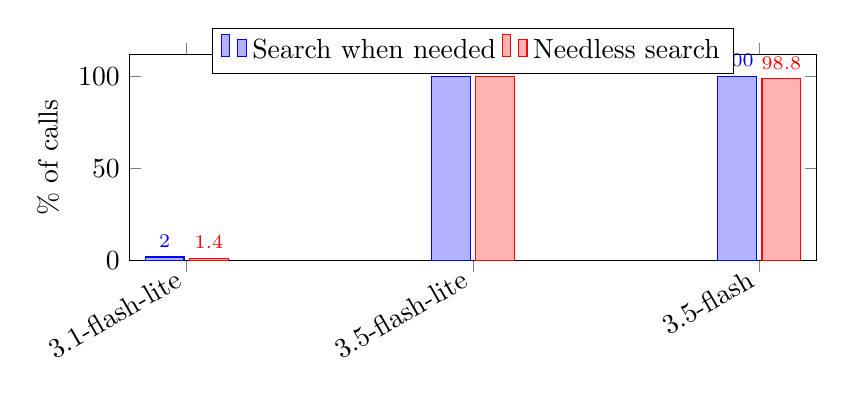
\begin{tikzpicture}
\begin{axis}[
  ybar, bar width=14pt,
  ymin=0, ymax=112,
  symbolic x coords={3.1-flash-lite,3.5-flash-lite,3.5-flash},
  xtick=data,
  x tick label style={rotate=30,anchor=east},
  ylabel={\% of calls},
  legend style={at={(0.5,1.13)},anchor=north,legend columns=-1},
  width=0.85\linewidth, height=4.2cm,
  nodes near coords, every node near coord/.append style={font=\scriptsize},
]
\addplot coordinates {(3.1-flash-lite,2.0) (3.5-flash-lite,100.0) (3.5-flash,100.0)};
\addplot coordinates {(3.1-flash-lite,1.4) (3.5-flash-lite,100.0) (3.5-flash,98.8)};
\legend{Search when needed, Needless search}
\end{axis}
\end{tikzpicture}
\caption{RQ1: search propensity is nearly binary, not calibrated — each model is either almost-never- or almost-always-search, independent of actual need.}
\label{fig:rq1}
\end{figure}

\texttt{gemini-3.1-flash-lite} searched in only 5 of 360 search-on calls in total; its on-condition performance is essentially identical to its off-condition performance. Both 3.5-generation models search on almost every call ($\sim$100\%) regardless of whether they already knew the answer. No model shows the calibrated "search only when needed" behavior that would be the ideal outcome — the 3.1$\to$3.5 gap is a \emph{tool-use propensity gap}, not a knowledge gap: the models did not get better at deciding whether to search, they simply moved from one uncalibrated extreme (never) to the other (always).

\subsection{RQ2: does a search tool change how the model handles fake IDs?}

\begin{table}[h]
\centering
\caption{RQ2: outcome on fake CVE IDs (\% of items), by search condition.}
\label{tab:rq2}
\footnotesize
\begin{tabular}{llccc}
\toprule
Model & Condition & Fabricated (\%) & Hijacked (\%) & Rejected (\%) \\
\midrule
gemini-3.1-flash-lite & off & 24.3 & 8.5 & 67.2 \\
                       & on  & 24.3 & 7.3 & 68.4 \\
gemini-3.5-flash-lite & off & 7.9 & 6.2 & 85.9 \\
                       & on  & 1.7 & 10.7 & 87.6 \\
gemini-3.5-flash       & off & 6.2 & 8.5 & 85.3 \\
                       & on  & 0.6 & 10.2 & 89.3 \\
\bottomrule
\end{tabular}
\end{table}

\begin{figure}[h]
\centering
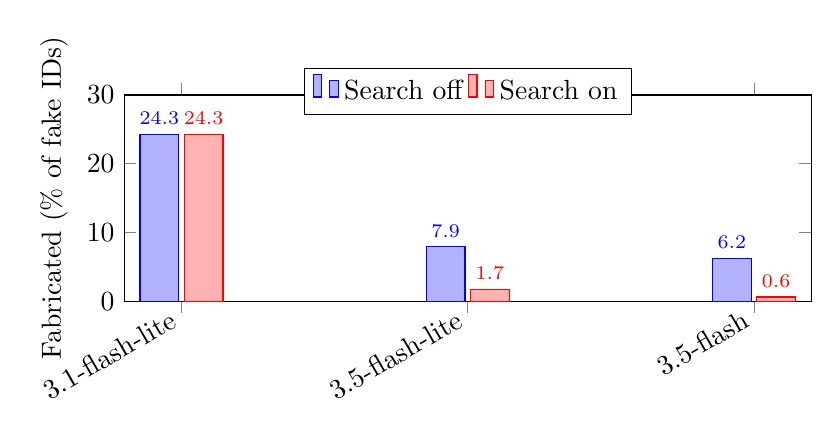
\begin{tikzpicture}
\begin{axis}[
  ybar, bar width=14pt,
  ymin=0, ymax=30,
  symbolic x coords={3.1-flash-lite,3.5-flash-lite,3.5-flash},
  xtick=data,
  x tick label style={rotate=30,anchor=east},
  ylabel={Fabricated (\% of fake IDs)},
  legend style={at={(0.5,1.13)},anchor=north,legend columns=-1},
  width=0.85\linewidth, height=4.2cm,
  nodes near coords, every node near coord/.append style={font=\scriptsize},
]
\addplot coordinates {(3.1-flash-lite,24.3) (3.5-flash-lite,7.9) (3.5-flash,6.2)};
\addplot coordinates {(3.1-flash-lite,24.3) (3.5-flash-lite,1.7) (3.5-flash,0.6)};
\legend{Search off, Search on}
\end{axis}
\end{tikzpicture}
\caption{RQ2: search availability roughly halves or more the fabrication rate on the two 3.5-generation models, but leaves \texttt{gemini-3.1-flash-lite} unchanged — consistent with it almost never actually searching (Figure~\ref{fig:rq1}).}
\label{fig:rq2}
\end{figure}

Search availability drives fabrication down substantially for both 3.5-generation models (e.g.\ \texttt{gemini-3.5-flash}: 6.2\%$\to$0.6\%) but has essentially no effect on \texttt{gemini-3.1-flash-lite}, which barely uses the tool. Hijacking, however, does \emph{not} fall with search — it stays flat or rises slightly across all three models.

This resistance to search is concentrated in one fake category. Table~\ref{tab:rq2near} splits hijacking by construction: \texttt{fake\_near\_miss} IDs (one digit off a real CVE) are hijacked far more often than \texttt{fake\_random} IDs, for every model and condition. That gap is the direct consequence of how the category is built — a near-miss ID sits one edit away from a real CVE that memory or search can retrieve and misattribute, while a random fake ID has no close, real neighbor to latch onto. Fabrication follows the same pattern (e.g.\ \texttt{gemini-3.1-flash-lite} fabricates \textasciitilde{}33\% of near-miss IDs vs.\ \textasciitilde{}16\% of random ones): near-miss IDs are simply harder to reject outright, not just more hijackable.

\begin{table}[h]
\centering
\caption{Hijack rate by fake-ID category (\% of items in that category).}
\label{tab:rq2near}
\footnotesize
\begin{tabular}{llcc}
\toprule
Model & Condition & Near-miss (\%) & Random (\%) \\
\midrule
gemini-3.1-flash-lite & off & 14.9 & 2.2 \\
                       & on  & 14.9 & 0.0 \\
gemini-3.5-flash-lite & off & 12.6 & 0.0 \\
                       & on  & 11.5 & 10.0 \\
gemini-3.5-flash       & off & 12.6 & 4.4 \\
                       & on  & 16.1 & 4.4 \\
\bottomrule
\end{tabular}
\end{table}

\subsection{RQ3: is self-reported confidence a useful signal?}

\begin{table}[h]
\centering
\caption{RQ3: mean self-reported confidence (0--100) by outcome, real IDs only.}
\label{tab:rq3}
\footnotesize
\begin{tabular}{lccc}
\toprule
Model & Correct & Declined & Wrong \\
\midrule
gemini-3.1-flash-lite & 99.9 ($n{=}177$) & 99.6 ($n{=}158$) & 93.6 ($n{=}25$) \\
gemini-3.5-flash-lite & 98.4 ($n{=}265$) & 99.2 ($n{=}85$) & 91.3 ($n{=}10$) \\
gemini-3.5-flash & 99.6 ($n{=}267$) & \textbf{29.0} ($n{=}88$) & 62.5 ($n{=}2$) \\
\bottomrule
\end{tabular}
\end{table}

All three models report high confidence ($\sim$98--100) on items they answer correctly — expected, since committing to a specific CVSS score or product list implies the model believes it has the facts. They diverge sharply on items they decline rather than commit to an answer: \texttt{gemini-3.5-flash}'s confidence drops to $\sim$29, while both lite-tier models still report $\sim$99 — the same near-maximal number they report everywhere else. Only \texttt{gemini-3.5-flash}'s confidence, then, tracks whether it actually has grounded content to offer; for the lite models the number barely moves regardless of outcome, so it carries little usable signal.

Declines are not an incidental subset: for every model, they occur almost exclusively on \texttt{real\_recent} items with search unavailable — the one case a model genuinely cannot know or check. This holds identically across models (so the confidence comparison is apples-to-apples), and it is why we do not split by condition: for \texttt{gemini-3.5-flash} and \texttt{gemini-3.5-flash-lite}, which search almost universally once available, a decline under search-on is essentially nonexistent — the tool converts those cases into a substantive answer instead.

\section{Discussion}

The headline result is that neither generation of models shows the target behavior — searching selectively, only when memory is insufficient. \texttt{gemini-3.1-flash-lite} almost never searches (2.0\% when it needs to); both 3.5-generation models almost always search (\textasciitilde{}100\%, including on items they already know). The apparent generational improvement in RQ2's fabrication numbers is therefore not evidence of better \emph{judgment} about when to search — it is what happens automatically once a model that searches unconditionally is given a tool that usually helps. This distinction matters practically: a model that always pays the latency/cost of a search call is a different (and more expensive) deployment story than one that has actually learned to decide.

Search is not a uniform fix, either. It suppresses outright fabrication but not hijacking — attaching a real, wrong CVE to a fake ID. This is arguably a worse failure mode in a security context: a fabricated answer is often easy to spot as ungrounded, while a hijacked answer comes with the trappings of a real, verifiable-looking CVE. Table~\ref{tab:rq2near} suggests why: hijacking concentrates on \texttt{fake\_near\_miss} IDs, which have a real CVE one edit away for memory or search to latch onto, so giving a model the ability to search does not, by itself, guarantee that it retrieves and uses the right thing.

Confidence is likewise not a reliable safety signal across the board. Only \texttt{gemini-3.5-flash}'s confidence score varies with what the model actually knows; the two lite-tier models report near-maximal confidence no matter what actually happened, so their confidence field carries no usable signal. Combined with the introspection failure noted in Section~\ref{sec:challenges} (weaker models misreporting their own tool use), this points to a broader pattern: self-reported signals from smaller/cheaper models — whether about confidence or about their own actions — should not be trusted at face value, even when the same signal is informative on a larger model in the same family.

\textbf{Limitations.} This study is Gemini-only; the original proposal's optional non-Google comparison was dropped, so we cannot say whether the search-propensity pattern is Gemini-specific or general. The hand-check that validates the LLM judge (Section~\ref{sec:scoring}) was done by a single human labeler, with no independent second annotator to compute inter-annotator agreement. We also did not test whether the model's thinking/reasoning budget affects fabrication rates — an early proposal aim scoped out once the core sweep and the Interactions-API migration (Section~\ref{sec:challenges}) consumed the available run budget. The confidence field (RQ3) also conflates confidence in the substantive answer with confidence in the choice to decline, so those results should be read as a within-model signal-strength comparison, not a claim about which confidence level is "correct" on a decline. Finally, the dataset (120 items) and the ground truth it depends on (NVD, MITRE) are a snapshot of a single day in a fast-moving landscape — one fake item in our set was itself published as a real CVE during the project, which we treat as a caution about how quickly "fake" and "real" can change under a live registry rather than as noise to be ignored.

\section{Code}

Code, dataset, and full experiment pipeline: \url{https://github.com/poratamit/cve_llm_eval} (branch \texttt{interactions-api}). The pipeline runs in six stages — \texttt{dataset/build\_dataset.py} $\to$ \texttt{harness/run\_experiment.py} $\to$ \texttt{scoring/score.py} $\to$ \texttt{scoring/handcheck.py} $\to$ \texttt{analysis/analyze.py} — each resumable and independently re-runnable against the committed \texttt{dataset/dataset.json}. The full sweep reported here (2{,}160 generations, $\sim$2{,}160 judge calls) cost well under \$100 in API spend (estimated $\sim$\$17).

\bibliographystyle{plainnat}
\bibliography{references}

\end{document}
